\chapter{Varietà e Spazi}
\section{Varietà differenziabile}
Le varietà differenziabili estendono il concetto di superficie noto in \R{3} a ipersuperfici di \R{n}. Viene introdotta una parametrizzazione generale di essa tramite l'uso di funzioni chiamate \textit{carte} che permettono di descrivere localmente la varietà (che a priori può essere curva o quant'altro), con un \textit{sistema di coordinate} in \R{n}. Inoltre le varietà permettono di svincolarsi dall'idea di \textit{immersione} in uno spazio a dimensione superiore, ideale per descrivere la struttura dello spaziotempo nella relatività generale.

\begin{definizione}
Una \textbf{varietà} (\textit{manifold}) $X$ è uno spazio topologico di Hausdorff in modo tale che ogni punto ha un intorno omeomorfo a \R{n}
\end{definizione}

Senza troppi dettagli ricordiamo che uno spazio topologico è un insieme dotato di una topologia che permette l'introduzione della nozione di intorno, di aperti, chiusi etc.
Uno spazio è di Hausdorff se per ogni coppia di punti è possibile definire due intorni di essi disgiunti.

\begin{definizione}
Una \textbf{carta} $(U,\phi)$ di una varietà $X$ è un insieme aperto $U\subset X$ (dominio) e un omeomorfismo $\phi : U \rightarrow V$, con $V\subset$ \R{n} aperto.

Le coordinate $(x^1,\dots,x^n)$ di $\phi(x)\in$ \R{n} del punto $x \in U \subset X$ vengono chiamate coordinate di $x$ sulla carta $(U,\phi)$.
\end{definizione}

Ricordiamo che un omeomorfismo è un'applicazione continua, biunivoca la cui inversa è anch'essa continua.

\begin{definizione}
Un \textbf{atlante} di classe $C^k$ su varietà $X$ è l'insieme di carte $\{(U_a, \phi_a)\}$ che coprono $X$ e con $\phi_a$ soddisfacenti:
\begin{equation*}
    \phi _b \circ \phi_a^{-1} : \phi_a(U_a \cap U_b) \rightarrow \phi _b(U_a \cap U_b)
\end{equation*}
di classe $C^k$ chiamate \textit{funzioni di transizione.}
\end{definizione}

In tal caso la varietà è differenziabile di ordine $C^k$.
Le carte permettono di definire la differenziabilità di una funzione sulla varietà.
\begin{figure}
    \centering
    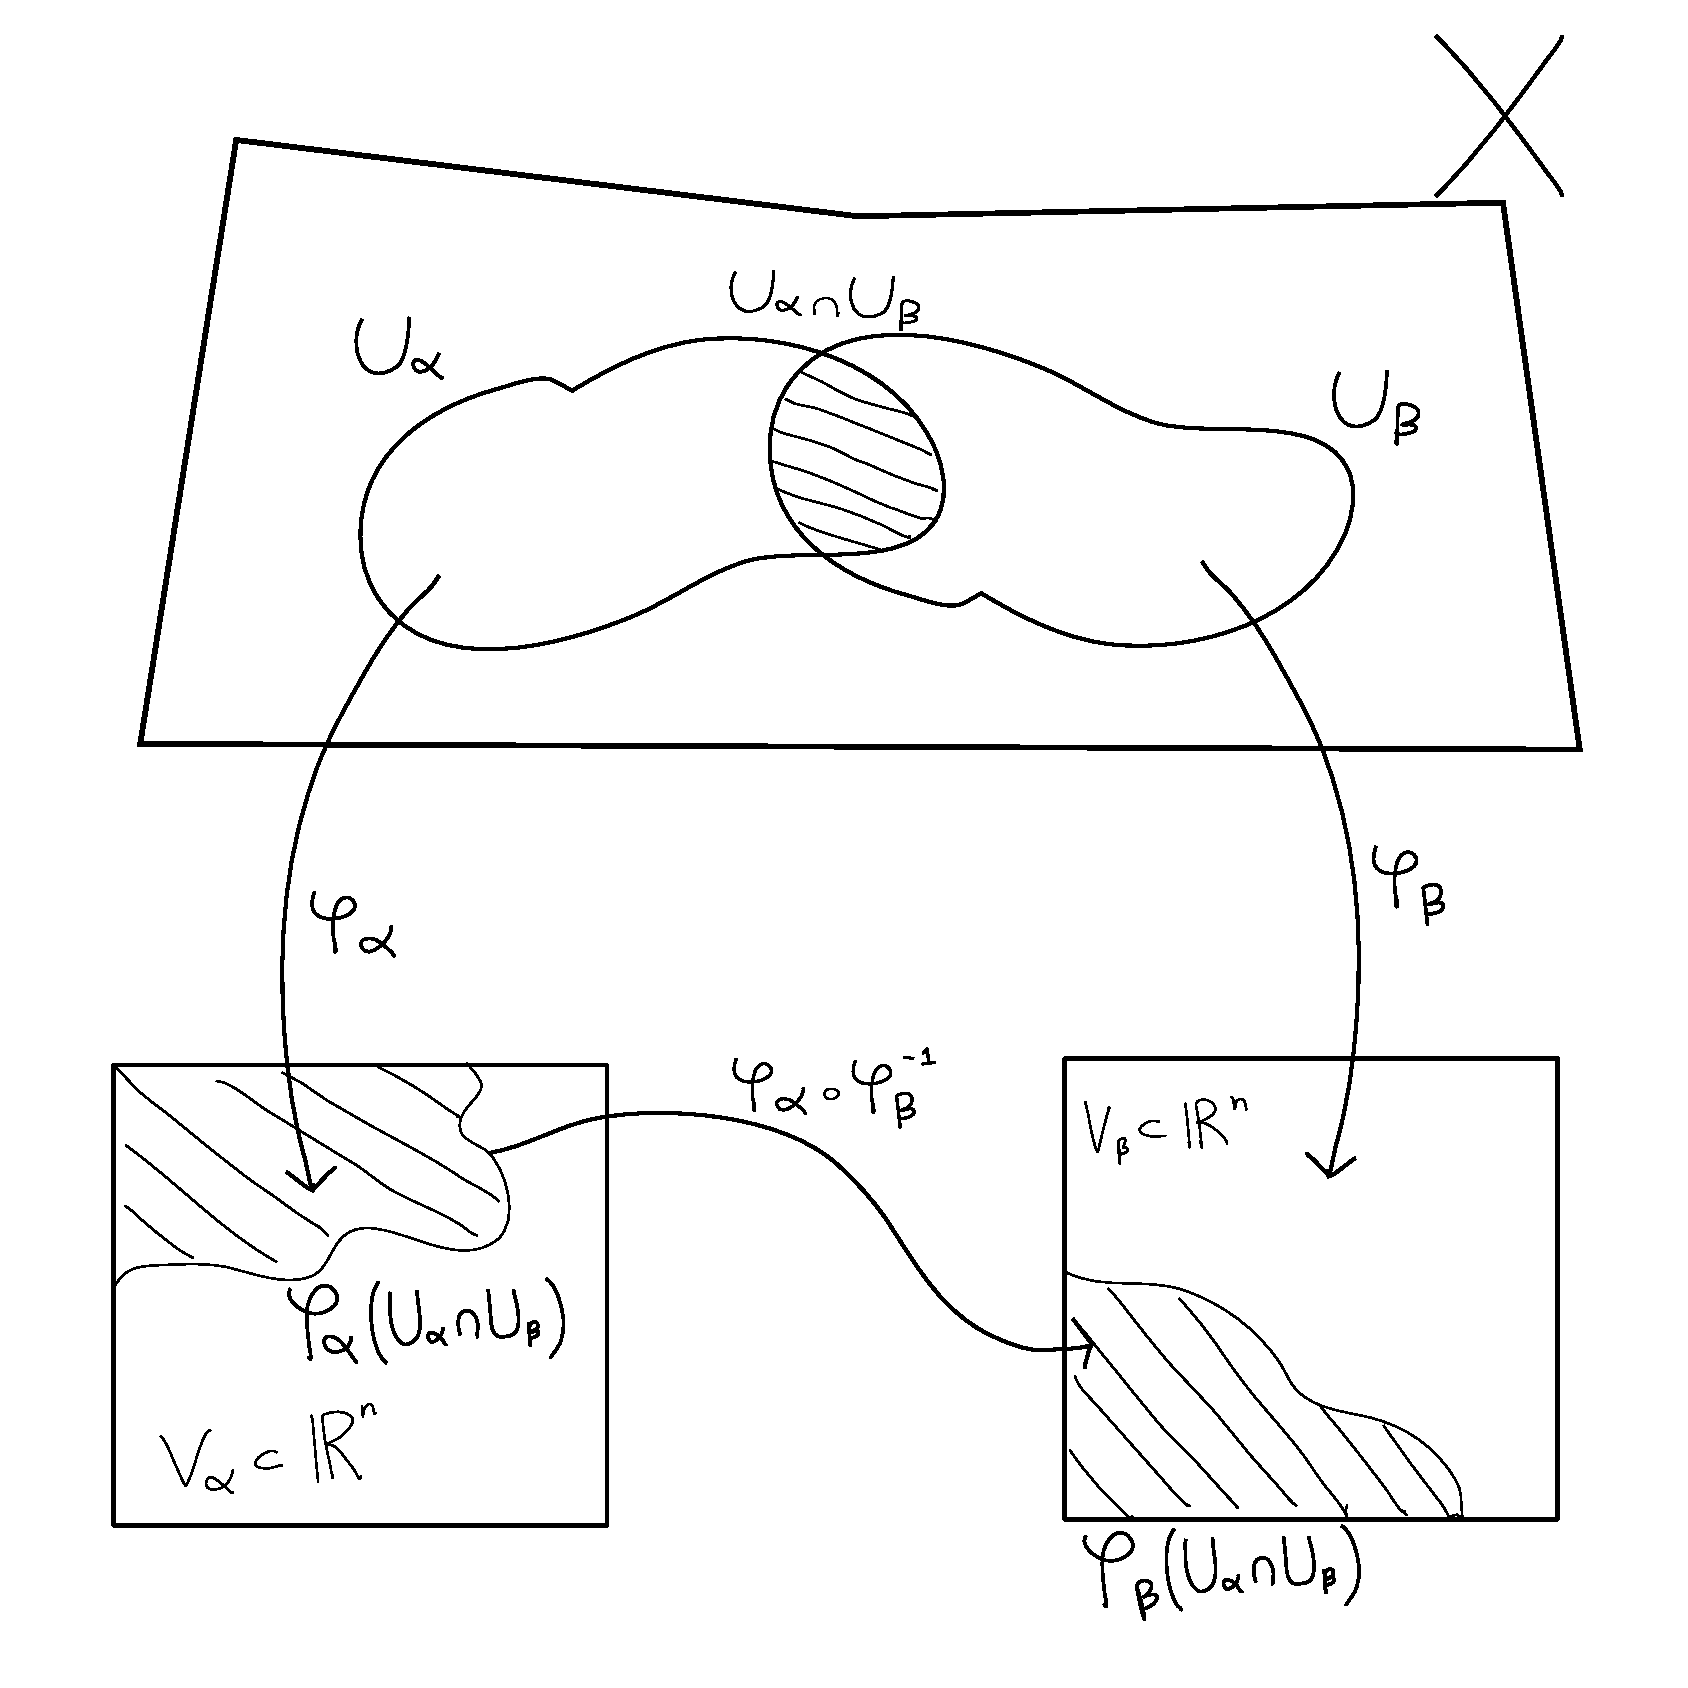
\includegraphics[scale=0.3]{immagini/atlante.pdf}
    \caption{Rappresentazione schematica di un atlante su una varietà con le funzioni di transizione.}
    \label{fig:my_label}
\end{figure}

\begin{definizione}
Sia una funzione $f : X \rightarrow \mathbb{R}$ e $x \in U$ tramite una carta $(U,\phi)$.
Si dice che la funzione \textbf{$f$ è differenziabile in $x$} $\in X$ se la funzione $f\circ \phi^{-1}: V=\phi(U) \subset \mathbb{R}^n \rightarrow \mathbb{R}$ è differenziabile in $\phi(x)$.
\end{definizione}

Così come $\phi(x)$ rappresenta localmente il punto $x$ nella carta $(U,\phi)$, la funzione $f\circ\phi^{-1}$ permette di rappresentare $f$ sulla carta locale.

Si osserva che la differenziabilità non dipende dalla carta, infatti:
\begin{equation*}
    f\circ \Tilde{\phi}^{-1} = (f \circ \phi^{-1})(\phi \circ \Tilde{\phi}^{-1})
\end{equation*}
dove $(f \circ \phi^{-1})$ è differenziabile per ipotesi e $(\phi \circ \Tilde{\phi}^{-1})$ è la funzione di transizione tra le due carte, quindi differenziabile.

\begin{definizione}
Siano $X^n, \ Y^p$ due varietà differenziabili di dimensione $n, \ p$ e $(U, \phi)$, $(W, \psi)$ due loro carte.
Sia $f: X^n \rightarrow Y^p$.
Si dice che $f$ è differenziabile in $x$ se $\psi \circ f \circ \phi^{-1}$ è differenziabile in $\phi(x)$.

$f$ è detto \textbf{diffeomorfismo} se è differenziabile, biettivo e la sua inversa differenziabile.
Riportiamo un teorema dell'analisi fondamentale per definire i diffeomorfismi locali:
\begin{teorema}
Sia $\Omega \subset \mathbb{R}^n$ aperto e $f=(f^1,\dots, f^n) :  \Omega \rightarrow \mathbb{R}^n$, $f\in C^1(\Omega)$. Sia $x_0 \in \Omega$, se det$(J_f(x_o))=$det$\frac{\partial(f^1,\dots, f^n)}{\partial(x_1,\dots, x_n)}(x_0)\neq 0$ allora $f$ è un diffeomorfismo locale.
\end{teorema}

\end{definizione}
La funzione $\psi \circ f \circ \phi^{-1}: \phi(U)\subset\mathbb{R}^n \rightarrow \psi(W)\subset\mathbb{R}^p$ rappresenta $f$ nelle due carte locali di $X, \ Y$.

I diffeomorfismi permettono di preservare la struttura differenziabile tra le varietà, così come gli omeomorfismi preservano la struttura topologica tra spazi topologici e gli isomorfismi la struttura algebrica.


\subsection{Spazio tangente, fibrato tangente, campo vettoriale}
Diamo per noto il concetto di vettori e spazio vettoriale (in particolare gli assiomi che devono essere soddisfatti e che definiscono tale spazio). Nella relatività ristretta lo spaziotempo di Minkowski ha una struttura naturale di spazio (piatto) 4-dimensionale, dove le operazioni di somma sono ben definite; tuttavia in geometrie curve la struttura di spazio vettoriale come nota, non è definita. Basti pensare a come non ci sia una nozione di somma tra vettori corrispondenti a punti diversi che garantiscano che il vettore somma appartenga alla varietà (pensa ad esempio ai punti di una sfera).

La nozione di spazio vettoriale potrà essere recuperata nel limite di spostamenti infinitesimi intorno ad un punto della varietà, introducendo cioè i vettori tangenti.
Inoltre nello sviluppo di una più generale definizione, dovremo come quanto fatto per le varietà, abbandonare l'idea di immersione in uno spazio superiore e per fare questo introdurremo la nozione di vettore tangente come derivata direzionale in un punto della varietà.\footnote{In $\mathbb{R}^n$ la corrispondenza tra vettori e derivate direzionali è uno a uno. Dato $v=(v^1,\dots, v^n)$ di definisce (e viceversa) $\sum_jv^j\partial/\partial x^j$}

\begin{definizione}
Sia $X$ una varietà, chiamiamo $\mathcal{F}$ la collezione di funzioni $ f \in C^\infty : X \rightarrow \mathbb{R} $.
\end{definizione}

\begin{definizione}
Sia $X$ una varietà, chiamiamo \textbf{vettore tangente a $p \in X$} la mappa $v : \mathcal{F} \rightarrow \mathbb{R}$ che soddisfa:
\begin{itemize}
    \item $v(af +bg) = av(f) + bv(g), \ \forall f,g \in \mathcal{F}; \forall a,b \in \mathbb{R}$ (linearità)
    \item $v(fg)= f(p)v(g) + g(p)v(f)$ (Leibniz)
\end{itemize}
Con le operazioni
\begin{itemize}
    \item $(v+w)(f) = v(f) + w(f)$
    \item $(av)(f) = av(f)$
\end{itemize}
i vettori tangenti acquisiscono la struttura di spazio vettoriale denominato \textbf{spazio tangente} a $p\in X$, $T_pX$.
\end{definizione}
Osserviamo che $v(\alpha) = 0$, $\forall \alpha \in \mathbb{R}$. Infatti usando la regola di Leibniz e imponendo $f=\alpha$ costante quindi usando la linearità per ogni $g$:
\begin{equation*}
    v(fg)=f(p)v(g) + g(p)v(f) \implies v(\alpha g) = \alpha v(g) = \alpha v(g) + g(p)v(\alpha) \implies g(p)v(\alpha)=0
\end{equation*}

Calcoliamo le componenti del vettore tangente.
Sia $f$ differenziabile in $x_0 \in X$ e sia $(U, \phi)$ una carta locale in $x_0$. Definendo $\Bar{f} = f \circ \phi^{-1}$ si ha $\Bar{f} : \phi(U) \rightarrow \mathbb{R}$ e pertanto
\begin{equation*}
    \Bar{f}(\phi(x)) = (f\circ \phi^{-1})(\phi(x)) = f(x)
\end{equation*}
Usando il teorema dell'incremento finito (o del valor medio) si ha che per qualche $s\in(0,1)$:
\begin{align*}
    f(x) &=\Bar{f}(\phi(x)) = \Bar{f}(\phi(x_0)) + \frac{\partial \Bar{f}}{\partial x^i} \Big|_{\phi(x_0) + s(\phi(x)-\phi(x_0))} (x^i -x_0^i)
\intertext{Sfruttando la funzione $\phi_i$ che estrae la $i$-esima coordinata:}    
    &=\Bar{f}(\phi(x_0)) + \frac{\partial \Bar{f}}{\partial x^i} \Big|_{\phi(x_0) + s(\phi(x)-\phi(x_0))} (\phi^i(x) -\phi^i(x_0))
\end{align*}
Chiamando per semplicità $\alpha = \Bar{f}(\phi(x_0))$, $\beta^i = \phi^i(x_0)$ e $g_i(x)=\frac{\partial \Bar{f}}{\partial x^i} \Big|_{\phi(x_0) + s(\phi(x)-\phi(x_0))}$ diventa:
\begin{equation*}
    f(x) = \alpha + g_i(x)(\phi^i(x) - \beta^i)
\end{equation*}
Riscritta in questo modo la funzione differenziabile iniziale, facciamoci agire il generico vettore tangente $v_x$ e sfruttiamo le proprietà della sua definizione:
\begin{align*}
    v_{x_0}(f) &= v_{x_0}(\alpha) + v_{x_0}(g_i(X)) (\phi^i(x_0) - \beta^i) + g^i(x_0)(v_{x_0}(\phi^i) - v_{x_0}(\beta^i)) \\
    &= g_i(x_0)v_{x_0}(\phi^i) = v^i \frac{\partial \Bar{f}}{\partial x^i}\Big|_{\phi(x_0)}
\end{align*}
avendo definito $v_{x_0}(\phi^i) = v^i$.

Data pertanto $f$ differenziabile, si definisce il vettore tangente in $x_0 \in X$ come
\begin{equation*}
    v_{x_0}(f) = v^i \frac{\partial \Bar{f}}{\partial x^i}\Big|_{\phi(x_0)}
\end{equation*}
di componenti $v^i$ e vettori di base $\frac{\partial}{\partial x^i} \equiv \partial_i$.

\begin{teorema}
I vettori $(\partial_1, \dots , \partial_n)$ formano una base dello spazio $T_x(X)$.
\end{teorema}
\proof{
La completezza è mostrata dal calcolo precedente. Tocca mostrare l'indipendenza lineare di tali vettori.
Sia $v_x(f) = v^i \frac{\partial \Bar{f}}{\partial x^i}|_{\phi(x)} = 0$ $\forall f$. Basta prendere $f= \phi^i$ la funzione che estrae la $i$-esima componente così che:
\begin{equation*}
    v_x(\phi^i) = 0 = v^i \implies  v^i = 0 \ \forall i
\end{equation*}\qed}

Per completezza, forniamo ulteriori definizioni della geometria differenziale strettamente connesse con la precedente.
\begin{definizione}
Chiamiamo \textbf{fibrato tangente} di una varietà $X$
\begin{equation*}
    TX = \bigcup_p T_p X
\end{equation*}
\end{definizione}
Se la varietà $X$ ha dimensione $n$, $p=(p^1,\dots, p^n)$ in una carta, un punto del fibrato viene individuato da un punto in $\mathbb{R}^{2n}$, $(p^1, \dots, p^n, v^1, \dots, v^n)$, cioè fornendo il punto e il vettore tangente ad esso.

\begin{definizione}
Chiamiamo \textbf{campo vettoriale tangente} alla varietà $X$ la funzione
\begin{equation*}
    F: X \rightarrow TX
\end{equation*}
che associa ad ogni $p \in X$, un elemento $F(p)\equiv v|_p \in T_p X$. Esso risulta una sezione del fibrato tangente.
\end{definizione}

In un sistema di coordinate locali, chiamato $n=dimX$, il campo vettoriale $F$ può essere definito nel dominio di una carta da $n$ funzioni $F^i$ (componenti) di $n$ variabili $x^1,\dots, x^n$.

Questa definizione in $\mathbb{R}^n$ può essere letta come \virgolette{un campo vettoriale è una funzione che associa ad un punto, un vettore}, in quanto la varietà e il suo spazio tangente coincidono.

Sia $f \in C^\infty$ una funzione liscia sulla varietà, allora per ogni $p\in X$ l'elemento $v|_p(f)$ è un numero e cioè $v(f)$ una funzione $X \rightarrow \mathbb{R}$.
\begin{definizione}
Diciamo che un campo vettoriale è \textbf{liscio} o regolare, se per ogni funzione $f\in C^\infty$, anche la funzione $v(f)$ è liscia o regolare sulla varietà.
\end{definizione}
Un campo vettoriale regolare può pertanto essere visto come un'applicazione:
\begin{equation*}
    F: \mathcal{F}(X) \rightarrow \mathcal{F}(X)
\end{equation*}
Qui i vettori tangenti sono stati definiti tramite \textit{derivazioni}.
Vediamo come tramite la nozione di flusso possiamo definire i vettori tangenti.
\begin{definizione}
Sia $X$ una varietà, un \textbf{gruppo di diffeomorfismi ad un parametro continuo} $\phi_t$ è una mappa $C^\infty$
\begin{equation*}
    \phi_t : \mathbb{R} \times X \rightarrow X
\end{equation*}
tale che per $t \in \mathbb{R}$ fissato, $\phi_t : X \rightarrow X$ è un diffeomorfismo e valgono per il parametro $t$ le regole di gruppo:
\begin{equation*}
    \phi_t \circ \phi_s = \phi_{t+s}
\end{equation*}
(segue che $\phi_0 = id$).
Per ogni $p\in X$ chiamiamo \textbf{orbita} di $\phi_t$, passante in $p$ a $t=0$, la mappa $\phi_t(p): \mathbb{R} \rightarrow X$ 
\end{definizione}
Il vettore tangente a $p$, $v|_p$\footnote{Viene usata indistintamente la notazione $v|_p$ e $v_p$.} è definito come la tangente alla curva a $t=0$, o più propriamente si identifica il vettore tangente a $p$ con la classe di equivalenza delle curve tangenti in $p$.
Si osserva che in tal modo stiamo definendo un campo vettoriale associato ad un gruppo a un parametro di trasformazioni di $X$ che può essere visto come il generatore infinitesimo delle trasformazioni.

\begin{esempio}
Un gruppo di Lie è una varietà differenziabile di funzioni analitiche che rispettino la struttura di gruppo. Lo spazio tangente all'identità di un gruppo di Lie viene chiamato algebra di Lie: i suoi elementi insieme ad una operazione bilineare antisimmetrica e che rispetti l'identità di Jacobi, chiamata parentesi di Lie, formano per l'appunto un'algebra.
\end{esempio}

Forniamo in maniera completa questa definizione alternativa di vettore tangente:
\begin{definizione}
Sia $C:I\subset \mathbb{R} \rightarrow X$, differenziabile in $X$ una curva tale che $C(0)=p$. Sia $f : X \rightarrow \mathbb{R}$, differenziabile in $p$, allora l'applicazione $f \circ C : I \rightarrow \mathbb{R}$ è differenziabile in $t=0$.

Definiamo il vettore tangente alla curva $C$ in $p$ la funzione $f \mapsto v|_p(f)$
\begin{equation*}
    v|_p(f) = \frac{d}{dt}(f\circ C)(t)|_{t=0}
\end{equation*}
chiamata derivata direzionale di $f$ lungo $C$ in $p$.
\end{definizione}
Se due curve $C_1, C_2$ sono tali che $v^{(C_1)}|_p(f) = v^{(C_2)}|_p(f)$, $\forall f$ allora si dicono tangenti in $p$. Ritorna quindi l'identificazione precedentemente detta con la classe di equivalenza delle curve tangenti nel punto.
\begin{figure}
    \centering
    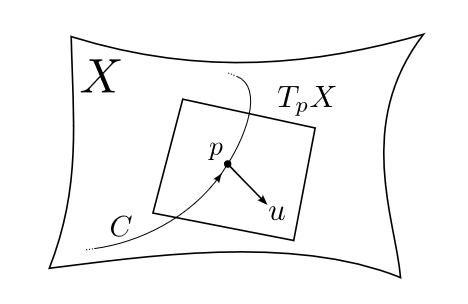
\includegraphics[scale=0.5]{immagini/vettangente.png}
    \caption{Vettore tangente ad una curva.}
    \label{fig.vett_tangente_curva}
\end{figure}

Un ultima definizione possibile di vettore tangente è anche:
\begin{definizione}
Un vettore tangente $v_p$ è una tripla $(p,\phi,v)$, con $\phi$ una carta, tale che $(p,\phi,v)$ e $(p,\phi', v')$ rappresentano lo stesso vettore se:
\begin{equation*}
    v' = D(\phi' \circ \phi^{-1})|_p v
\end{equation*}
dove $D(\phi' \circ \phi^{-1})$ è la matrice Jacobiana nella trasformazione tra $v$ e $v'$, ovvero la matrice di componenti:
\begin{equation*}
    J_{ji}(\phi(p)) = \frac{\partial x'^j}{\partial x^i}\Big|_{\phi(p)}
\end{equation*}
\end{definizione}
Quest'ultima definizione equivale a dire che il vettore tangente trasforma come un vettore tramite la trasformazione tra le carte.

\begin{definizione}
Sia $F$ un campo vettoriale regolare sulla varietà $X$. Una curva $\alpha : (a,b) \rightarrow X$ è detta \textbf{curva integrale} di $F$ se
\begin{equation*}
    \Dot{\alpha}(t) = F(\alpha(t)) \ \ \forall t \in (a,b)
\end{equation*}
cioè per ogni punto ha come vettore tangente il campo vettoriale.
\end{definizione}
In particolar modo esistono teoremi di esistenza e unicità delle curve integrali dato un campo vettoriale:
\begin{teorema}
Sia $F$ un campo vettoriale regolare su $X$ e $p \in X$, allora $\exists (a,b)$ e la curva:
\begin{equation*}
    \alpha_p(t) : (a,b) \rightarrow X
\end{equation*}
tali che:
\begin{enumerate}
    \item $\alpha_p(0) = p$
    \item $\alpha_p$ è curva integrale di $F$
    \item $\alpha_p$ è curva massimale, quindi se esiste $\beta :(c,d)\rightarrow X$ e soddisfa i precedenti punti, allora $(c,d) \subset (a,b)$
\end{enumerate}
\end{teorema}
In generale l'intervallo $(a,b)$ dipende dal punto $p$.
\begin{definizione}
    Un campo vettoriale $F$ viene detto \textbf{completo} se il dominio di $\alpha_p$ è $\mathbb{R}$ $\forall p \in X$
\end{definizione}

Per le curve integrali si può ottenere in generale un'equazione differenziale al primo ordine che lega la curva integrale al campo vettoriale. Questa può essere risolta per determinare se il campo è completo, ad esempio.
Se prendiamo la definizione di vettore tangente ad una curva, e l'applichiamo sulle funzioni delle coordinate $x_i = r_i \circ \phi$ dove $r_i$ è la proiezione in $\mathbb{R}^n$ e $\phi$ una mappa delle coordinate, facendo per componenti:
\begin{equation*}
    \Dot{\alpha}(t) = \sum \frac{d(x_i \circ \alpha)}{dt}\frac{\partial}{\partial x_i}\Big|_{\alpha(t)} = F(\alpha(t)) = \sum F^i(\alpha(t)) \frac{\partial}{\partial x_i}\Big|_{\alpha(t)}
\end{equation*}
poiché $(x_i \circ \alpha)(t)= \alpha^i(t)$, ottiene:
\begin{equation*}
    \frac{d\alpha^i(t)}{dt} = F^i(\alpha(t))
\end{equation*}
\subsection{Spazio cotangente}
\'E utile in geometria differenziale introdurre anche il differenziale di una funzione, quale applicazione che permette di mappare uno spazio tangente ad un punto di una varietà, nel tangente in un'altra varietà.
\begin{definizione}
    Data una funzione $f: X \rightarrow Y$, tra le due varietà $X, Y$ e dato un punto $p \in X$, definiamo il \textbf{differenziale} di $f$ in $p$:
\begin{equation}
        df: T_pX \rightarrow T_{f(p)}Y
        \label{eq.differenziale}
\end{equation}
come la funzione che, dato $v \in T_pX$, allora $df(v)$ è l'elemento di $T_{f(p)}Y$ che agisce sulle funzioni $g\in\mathcal{F}(Y)$ secondo:
\begin{equation*}
    df(v): g \mapsto v(g\circ f)
\end{equation*}
\end{definizione}
Al variare di $v \in T_pX$, fissando $f$ e $g$ , la funzione lineare $df$ è un elemento del duale dello spazio tangente.

\begin{definizione}
Definiamo lo \textbf{spazio cotangente} di $T_pX$ lo spazio duale dello spazio tangente, ovvero lo spazio dei funzionali lineari
\begin{align*}
    \omega_p : T_pX &\rightarrow \mathbb{R}\\
    v_p &\mapsto \omega_p(v)
\end{align*}
\end{definizione}

Sia $\{e_i\}$ base dello spazio $T_pX$ e $v_p=(v_p^1, \dots, v_p^n)$ le componenti di un vettore tangente in essa, determiniamo la sua base duale. Possiamo definire il funzionale $\theta^i(v_p)=v_p^i$ e in tal modo otteniamo la relazione
\begin{equation*}
    \theta^i(v_p^je_j) = v_p^j\theta^i(e_j) \equiv v_p^i \iff \theta^i(e_j)= \delta^i_j
\end{equation*}
Di fatto l'azione della $i$-esima componente di base dello spazio cotangente è l'estrazione della $i$-esima componente del vettore tangente.

Chiamiamo la base naturale dello spazio cotangente $\{dx^i\}$, la base duale di $\{\partial_j\}$ i.e. $dx^i(\partial_j)=\delta^i_j$. Si usa anche annotare lo spazio cotangente con $T_p^*X$.
\subsection{Cambiamenti di base: covarianza e controvarianza}
Sia la trasformazione tra due diverse basi dello spazio tangente:
\begin{equation}
    e_i= \tensor{a}{_i ^k} e'_k
    \label{eq.basetransvett}
\end{equation}
La trasformazione delle componenti risulta:
\begin{equation*}
    v= v^i e_i = v^i \tensor{a}{_i ^k} e'_k = v'^k e'_k
\end{equation*}
Le componenti sono dette \textbf{controvarianti} e indicate con indice alto se trasformano secondo:

\begin{equation}
    v'^k = v^i \tensor{a}{_i^k}
    \label{eq.contrav}
\end{equation}
cioè inversamente alla trasformazione della base.

Possiamo determinare così la trasformazione degli elementi della base duale:
\begin{equation*}
    \theta'^k(v) = v'^k = v^i \tensor{a}{_i^k} = \theta^i(v)  \tensor{a}{_i^k}
\end{equation*}
cioè
\begin{equation}
     \theta'^k = \theta^i  \tensor{a}{_i^k}
     \label{eq.basetranscovett}
\end{equation}
La base duale trasforma con l'inverso della trasformazione della base ${e_i}$.
La trasformazione delle componenti risulta:
\begin{equation*}
     \omega = \omega_i \theta^i = \omega_i \tensor{(a^{-1})}{_k^i} \theta'^k = \omega'_k \theta'^k
\end{equation*}
Le componenti sono dette \textbf{covarianti} e indicate con indice basso se trasformano secondo:

\begin{equation}
     \omega'_k = \tensor{(a^{-1})}{_k^i} \omega_i
     \label{eq.covar}
\end{equation}

Utilizzando la base naturale, $e_i =\partial_i$, $\theta^i=dx^i$ e considerando il cambio di base indotto dal cambio di coordinate, cioè della carta adottata ($x^i \rightarrow x'^i$):
\begin{equation*}
    \frac{\partial}{\partial x^i} = \frac{\partial x'^j}{\partial x^i}\frac{\partial}{\partial x'^j} \iff \partial_i = \frac{\partial x'^j}{\partial x^i} \partial'_j
\end{equation*}
dove la matrice $\frac{\partial x'^j}{\partial x^i}$ non è altro che lo jacobiano della trasformazione di coordinate.
Questo induce la trasformazione sul duale:
\begin{equation*}
    dx'^i = \frac{\partial x'^i}{\partial x^j} dx^j
\end{equation*}
a dimostrare che effettivamente è il differenziale di $x'$.
